%%%%%%%%%%%%%%%%%%%%%%%%%%%%%%%%%%%%%%%%
% Class options                        %
%%%%%%%%%%%%%%%%%%%%%%%%%%%%%%%%%%%%%%%%
% Orientation:                         %
% portrait (default), landscape        %
%                                      %
% Paper size:                          %
% a0paper (default), a1paper, a2paper, %
% a3paper, a4paper, a5paper, a6paper   %
%                                      %
% Language:                            %
% english (default), norsk             %
%%%%%%%%%%%%%%%%%%%%%%%%%%%%%%%%%%%%%%%%
\documentclass{uioposter}


\usepackage{lipsum}                                % Dummy text
\usepackage[figwidth = 0.98\linewidth]{todonotes}  % Dummy image (and more!)
\usepackage[absolute, overlay]{textpos}            % Figure placement
\usepackage{hyperref}
% \usepackage{fontspec}

% \setsansfont[Ligatures=TeX]{Raleway}
% \setsansfont[Ligatures=TeX]{Arial}

\setlength{\TPHorizModule}{\paperwidth}
\setlength{\TPVertModule}{\paperheight}

\newcommand{\etal}{\emph{et al. }}


\title{Applications of Machine Learning to Soft Matter}
\author
{%
    Edwin Bedolla\inst{1, $\dagger$}
    \and
    Edmundo Vázquez\inst{1}
    \and
    Ramón Castañeda-Priego\inst{1,2}
}
%% Optional:
\institute
{
    \inst{1} División de Ciencias e Ingenierías
    \and
    \inst{2} Departamento de Ingeniería Física
}
% Or:
%\institute{Contact information}


%% Remove footline:
\setbeamertemplate{footline}{}


\begin{document}
\begin{frame}
\begin{columns}[onlytextwidth]


\begin{column}{0.5\textwidth - 1.5cm}
    \begin{alertblock}{Abstract}
        With recent developments in Machine Learning (ML) technology, Soft Matter (SM) has been adopting several methodologies to enhance and provide new insights into difficult problems within the field. In this work, we showcase two recent applications of ML to SM systems, namely a data-driven ML model to show how structure is important to glassy dynamics; and a Deep Learning techinique to train ML models in order to detect topological defects in liquid crystals with data from video microscopy experiments. We briefly discuss the advantages and shortcomings of these frameworks, with the hope that future research can adopt some of these ideas and techniques in order to empower problem solving within SM.
    \end{alertblock}

    % \begin{block}{Introduction}
    %     Within the Condensed Matter Physics field, Machine Learning (ML) is currently used in several research areas, ranging from
    %     quantum matter~\cite{carrasquilla_2020}, solid state physics~\cite{schmidt2019recent}, and more importantly, Soft Matter (SM). 
    %     The need to use ML is directly related to the amount of data that usual techniques
    %     create, in the form of experiments and computer simulations.
    %     Furthermore, there is a motivation that by using ML models, coupled with physics-designed
    %     features, new insights and physical parameters can be found from the datasets.
    %     For a more complete overview of the topic, we
    %     refer the reader to a recent review~\cite{bedolla2020}.

    %     Most of the applications that have been used deal almost exclusively with
    %     Hard Matter systems, such as spin systems like the $XY$ model, the Potts model,
    %     the Ising model, and others. This fact is due to ML models being developed
    %     mainly for grid-like data, such as images in computer vision. 
    %     Due to the fact that spin systems are grid-like data, ML models can be
    %     readily applied to them, although care must be taken when training and other
    %     technical details to ensure that the results obtained are physicaly meaningful
    %     and correct.

    %     On the other hand, SM has seen very little applications due
    %     to the fact that modern ML technology does not handle off-lattice and
    %     continuous data easily. Nevertheless, some work has been carried out
    %     in developing carefuly crafted features from simulation and experimental
    %     data that have boosted ML applications in the field of SM.
    % \end{block}

    \begin{block}{Structure and glassy dynamics}
        In a recent paper~\cite{glassy2016}, Schoenholz \etal discovered that structure
        is an important physical feature to glassy dynamics in three dimensions. By
        separating particles into two main classes, either \emph{soft} or \emph{hard},
        they defined a \emph{softness} parameter using a classifier to accomplish such task.

        A particle is determined as soft if it is likely to rearrange, and hard otherwise.
        These parameters are defined through "structure functions"~\cite{behler2007generalized}
        that preserve the overall isotropic symmetry of the system
        and include radial density and bond angle information. These functions serve as the
        feature vectors, and a training set is built with this information. Using a particular
        classifier called a Support Vector Machine (SVM)~\cite{friedman2001elements},
        the softness of a particle $i$, $S_i$, is defined as the shortest distance between its position
        in the feature space span by the corresponding feature vectors, and the hyperplane
        that separates both clases, either soft, when $S_i > 0$ or hard, $S_i < 0.$

        \begin{figure}
            \centering
            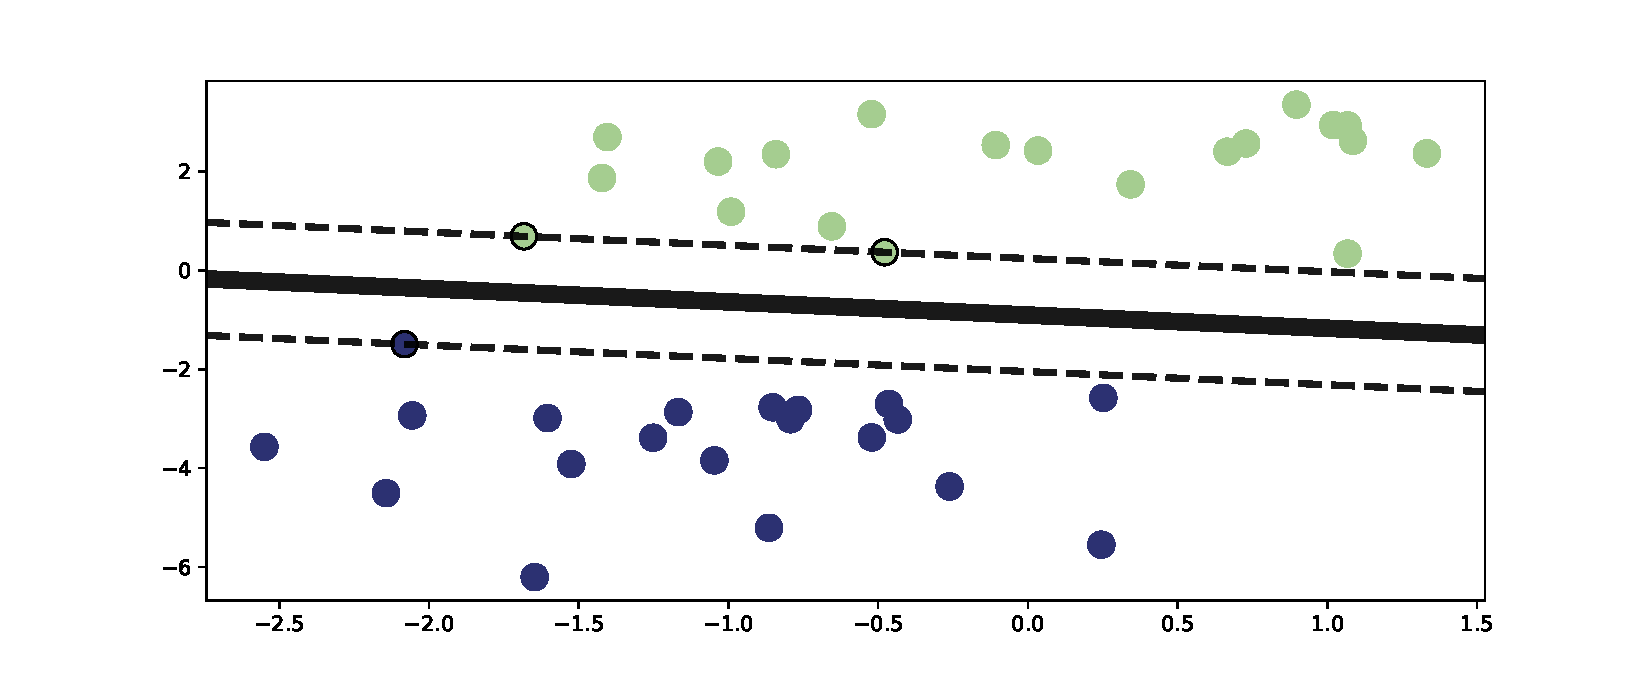
\includegraphics[width=0.8\textwidth]{uioposter-images/fig2.pdf}
        \end{figure}

        It is important to note here that SVMs are ML models that do not scale well with
        large datasets, but the main takeaway of such models is that its formulation
        is mathematically rigorous and well understood. Here, the important aspect of
        using a SVM is to give meaning to the classification mechanism of such models
        in a physical problem.
    \end{block}

    \begin{alertblock}{References}
        \begin{thebibliography}{99}
            \bibitem{carrasquilla_2020}
            Carrasquilla, J.,
            Machine learning for quantum matter,
            \emph{Advances in Physics: X},
            5, pp. 1797528, 2020.
            
            \bibitem{schmidt2019recent}
            Schmidt, J., and Marques, M. and Botti, S. and Marques, M. AL.,
            Recent advances and applications of machine learning in solid-state materials science,
            \emph{npj Computational Materials},
            5, pp. 1-55, 2019.
            
            \bibitem{bedolla2020}
            Bedolla, E., and Padierna, L.C., and Casta{\~n}eda-Priego, R.,
            Machine Learning for Condensed Matter Physics,
            \emph{Journal of Physics: Condensed Matter},
            2020.

            \bibitem{friedman2001elements}
            Friedman, J., and Hastie, T., and Tibshirani, R.,
            \emph{The elements of statistical learning},
            first ed., Springer series in statistics New York, 2001.

            \bibitem{glassy2016}
            Schoenholz, S., Cubuk, E., Sussman, D. \etal,
            A structural approach to relaxation in glassy liquids,
            \emph{Nature Physics},
            12, 469–471, 2016.

            \bibitem{behler2007generalized}
            Generalized neural-network representation of high-dimensional
            potential-energy surfaces,
            Behler, J., and Parrinello, M.,
            \emph{Physical Review Letters},
            98, 14, pp. 146401, 2007.

            \bibitem{endtoend2020}
            Minor, Eric N., and Howard, S. D., and Green, A. A. S., and Glaser, M. A., and Park, C. S., and Clark, N. A.,
            End-to-end machine learning for experimental physics: using simulated data to train a neural network for object detection in video microscopy,
            \emph{Soft Matter},
            16, 7, 1751-1759, 2020.
            \end{thebibliography}
    \end{alertblock}

\end{column}


\begin{column}{0.5\textwidth - 1.5cm}
    \begin{block}{Deep Learning and Video Microscopy}
        \begin{figure}
            \centering
            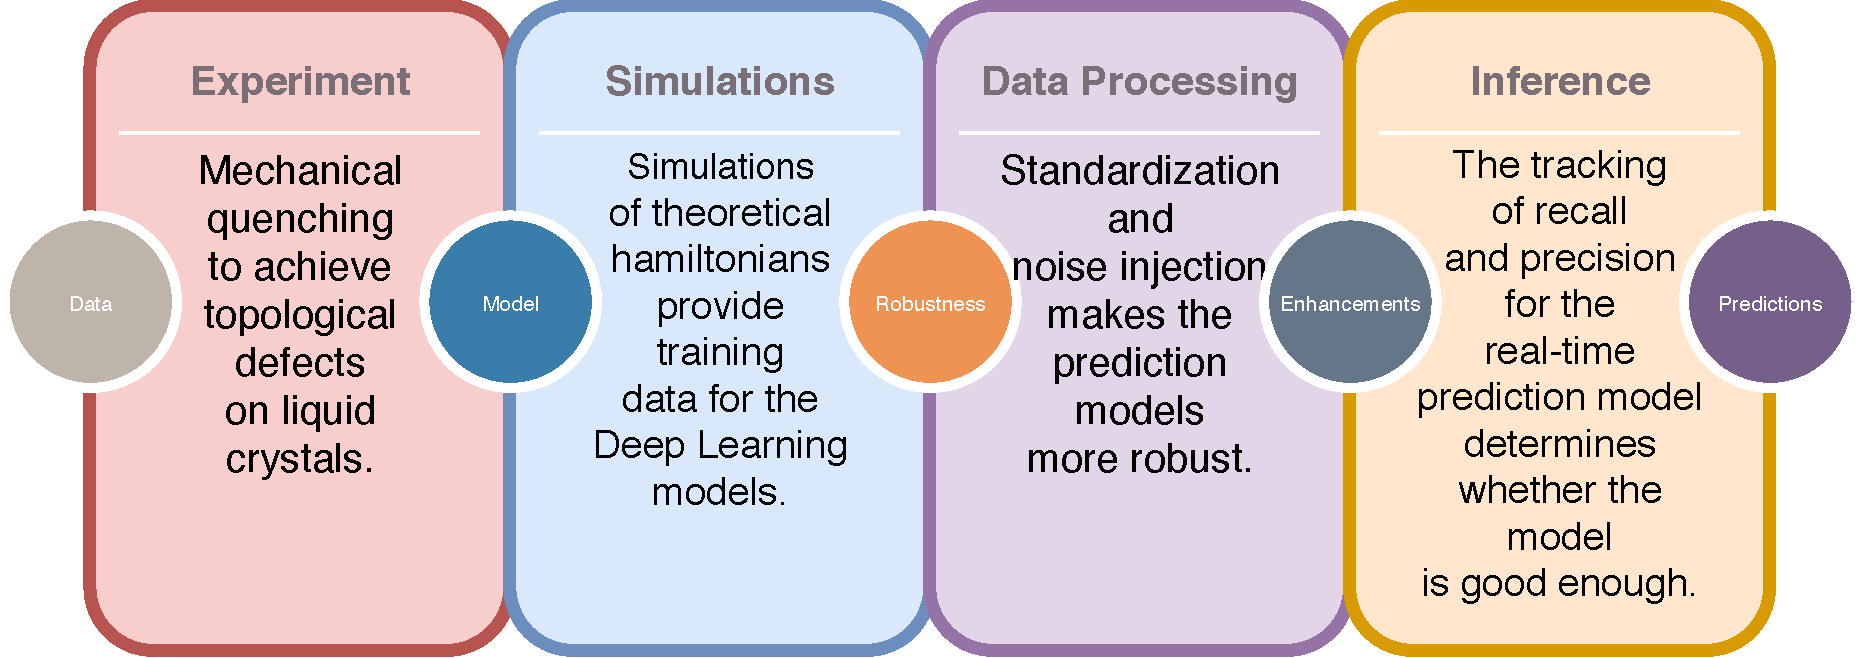
\includegraphics[width=0.85\textwidth]{uioposter-images/fig1.pdf}
        \end{figure}

        ML technology has also aided the development of robust and fast experimental
        setups. One such example was developed by Minor \etal~\cite{endtoend2020} in a recent work where
        an end-to-end ML framework, together with simulation data, was created in order
        to provide an accurate study of topological defect annhilation in liquid
        crystals.

        The complete framework consists of a typical topological defect experiment
        using a mechanical quencher and video microscopy. In the experiment, the liquid
        crystal is always ensured to be on the smectic phase. This will provide some of the \emph{testing data},
        a dataset that will no be used as input into the ML model.
        Instead, simulation of the $XY$ model is carried out, with randonmly placed
        topological defects. With this new dataset, together with a subset of the
        video microscopy data, will comprise the full traning dataset.

        One of the most important outcomes of this methodology is the fact that by having
        trained a ML model with enough robustness, the same apparatus can be used with
        different topological defects, with minimal modification of the ML model.
        This constitutes an important achievement in the sense that modern ML frameworks
        can be used not only with simulation data, but with experimental data as well.
    \end{block}

    \begin{exampleblock}{Discussions}
        % TODO: Completar las perspectivas y discusiones
    \end{exampleblock}

    \begin{exampleblock}{Acknowledgements}
        This work was financially supported by Conacyt grant 287067.
    \end{exampleblock}

    
\end{column}


\end{columns}


\end{frame}
\end{document}